\chapter{Aplicaciones entre Espacios Topológicos}

\section{Continuidad}

Para $\bb{R}$, decíamos que $f:\bb{R}\to \bb{R}$ es continua en $x_0\in \bb{R}$ si:
\begin{equation*}
    \forall \veps\in \bb{R}^+,~\exists \delta\in \bb{R}^+ \mid \forall x \text{ con } |x-x_0|<\delta \text{ se tiene que } |f(x)-f(x_0)|<\veps
\end{equation*}

Para espacios métricos, decíamos que dada $f:(X,d)\to (Y,d')$ es continua en $x_0\in X$ si:
\begin{equation*}
    \forall \veps\in \bb{R}^+,~\exists \delta\in \bb{R}^+ \mid f[B(x_0,\delta)]\subset B[f(x_0,\veps)]
\end{equation*}

Esto es equivalente a decir que:
\begin{equation*}
    \forall N\in N_{f(x_0)} \text{ se tiene que } f^{-1}(N)\in N_{x_0}
\end{equation*}

\begin{observacion}
    Recordamos las siguientes nociones de Álgebra I. Sea $f:X\to Y$. Entonces, dado $W\subset X$, $Z\subset Y$, se tiene que:
    \begin{enumerate}
        \item $W\subset f^{-1}(f(W))$. Además, si es inyectiva se da la igualdad.

        \item $f^{-1}(f(Z))\subset Z$. Además, si es sobreyectiva se da la igualdad.
    \end{enumerate}
\end{observacion}

Esta definición se generaliza para cualquier espacio topológico:
\begin{definicion}[Continuidad]
    Sea $f:(X,\T)\to (Y,\T')$ una aplicación entre dos espacios topológicos, y sea $x_0\in X$. Decimos que $f$ es continua en $x_0$ si para todo $N'\in N_{f(x_0)}$ entorno de $f(x_0)$ existe un entorno $N\in N_{x_0}$ entorno de $x_0$ tal que $f(N)\subset N'$. Es decir,
    \begin{equation*}
        \forall N'\in N_{f(x_0)},~~\exists N\in N_{x_0} \text{ con } f(N)\subset N'
    \end{equation*}
\end{definicion}


Vamos a caracterizar la definición de continuidad en términos de bases, bases de entornos y también en términos de la preimagen de $f$:
\begin{prop}[Caracterización de la continuidad]\label{prop:Caract_ContinuidadPto}
    Sea $f:(X,\T)\to (Y,\T')$ una aplicación entre dos espacios topológicos, y sea $x_0\in X$. Entonces, son equivalentes:
    \begin{enumerate}
        \item $f$ es continua en $x_0$.
        \item Dadas $\beta_{x_0}$ base de entornos de $x_0$ y $\beta_{f(x_0)}$ base de entornos de $f(x_0)$, para cualquier $V'\in \beta_{f(x_0)}$ existe $V\in \beta_{x_0}$ tal que $f(V)\subset V'$. Es decir,
        \begin{equation*}
            \forall V'\in \beta_{f(x_0)},~~\exists V\in \beta_{x_0} \mid f(V)\subset V'
        \end{equation*}
        \item La preimagen de cualquier entorno de $f(x_0)$ es un entorno de $x_0$. Es decir,
        \begin{equation*}
            \forall N\in N_{f(x_0)}\text{ se tiene que } f^{-1}(N)\in N_{x_0}
        \end{equation*}
    \end{enumerate}
\end{prop}
\begin{proof}\
    \begin{description}
        \item[$1\Longrightarrow 2)$] Dado $V'\in \beta_{f(x_0)}$, en particular $V'\in N_{f(x_0)}$. Como $f$ es continua en $x_0$ se tiene que $\exists N\in N_{x_0}$ tal que $f(N)\subset V'$. 
        
        Por ser $\beta_{x_0}$ una base de entornos, por definición $\exists V\in \beta_{x_0}$ tal que $V\subset N$. Por tanto, se tiene que $f(V)\subset f(N)\subset V'$, demostrando así 2).
    
        \item[$2\Longrightarrow 3)$] Consideramos las bases de entornos triviales dadas por todos los entornos. Entonces, dado $N\in N_{f(x_0)}=\beta_{f(x_0)}$, por 2) se tiene que $\exists V\in N_{x_0}=\beta_{x_0}$ tal que $f(V)\subset N$.
        
        Entonces, $V\subset f^{-1}(f(V))\subset f^{-1}(N)$. Como $V\in N_{x_0}$, y $V\subset f^{-1}(N)$, tenemos que $f^{-1}(N)\in N_{x_0}$.

        \item[$3\Longrightarrow 1)$] Dado $N'\in N_{f(x_0)}$, por 3) tenemos que $f^{-1}(N')\in N_{x_0}$. Consideramos $N=~f^{-1}(N')$. Entonces $f(N)=f(f^{-1}(N'))\subset N'$, por lo que tenemos que $f$ es continua en $x_0$.
    \end{description}
\end{proof}

\begin{definicion}[Continuidad global] Sea $f:(X,\T)\to (Y,\T')$ una aplicación entre espacios topológicos. Decimos que $f$ es continua si $f$ es continua en todo $x\in X$.
\end{definicion}

\begin{prop}[Caracterización de la continuidad global]\label{prop:Caract_ContinuidadGlobal}
    Sea $f:(X,\T)\to (Y,\T')$ una aplicación entre dos espacios topológicos. Entonces, son equivalentes:
    \begin{enumerate}
        \item $f$ es continua.
        \item La preimagen de todo abierto de $\T'$ es un abierto de $\T$. Es decir,
        \begin{equation*}
            f^{-1}(U')\in \T, \qquad \forall U'\in \T'
        \end{equation*}
        \item La preimagen de todo abierto básico (de una base dada) es abierto. Es decir, dada $\cc{B}'$ base de $\T'$, se cumple que:
        \begin{equation*}
            f^{-1}(B')\in \T, \qquad \forall B'\in \cc{B}'
        \end{equation*}

        \item La preimagen de todo elemento de una subbase fijada de $\T'$ es un abierto. Es decir, dada $S$ subbase de $\T'$, se tiene que:
        \begin{equation*}
            f^{-1}(A)\in \T, \qquad \forall A\in S
        \end{equation*}

        \item La preimagen de todo cerrado de $\T'$ es un cerrado de $\T$. Es decir,
        \begin{equation*}
            f^{-1}(C)\in C_\T, \qquad \forall C'\in C_{\T'}
        \end{equation*}

        \item Dado $D\subset X$, la imagen de su adherencia ha de estar contenida en la adherencia de su imagen. Es decir,
        \begin{equation*}
            f(\ol{D})\subset \ol{f(D)},\qquad \forall D\subset X
        \end{equation*}
    \end{enumerate}
\end{prop}
\begin{proof}\
    \begin{description}
        \item[$1\Longrightarrow 2)$] Dado $U\in T'$, por la Proposición \ref{prop:CaractAbiertos_conEntornos}, tenemos que $U\in N_x~\forall x\in U$. En particular, dado $x_0\in f^{-1}(U)\subset X$, como $U\in N_{f(x_0)}$ y $f$ es continua en $x_0$, tenemos que $f^{-1}(U)\in N_{x_0}$.

        Por tanto, tenemos que $f^{-1}(U)\in N_{x_0}~\forall x_0\in f^{-1}(U)$. Por tanto, por la proposición \ref{prop:CaractAbiertos_conEntornos}, tenemos que $f^{-1}(U)\in \T$, quedando demostrada esta implicación.

        \item[$2\Longrightarrow 1)$] Tenemos que probar que $f$ es continua; es decir, si $x_0\in X$, entonces $f$ es continua en $x_0$.

        Dado $x_0\in X$, por la Proposición \ref{prop:Caract_ContinuidadPto}, tenemos que demostrar que si $N\in N_{f(x_0)}$, entonces $f^{-1}(N)\in N_{x_0}$.

        Como $N\in N_{f(x_0)}$, $\exists U\in \T'$ tal que $f(x_0)\in U\subset N$. Entonces, usando 2) tenemos que $x_0\in f^{-1}(f(x_0))\subset f^{-1}(U)\subset f^{-1}(N)$ entorno de $x_0$.

        TERMINAR



        \item[$2\Longrightarrow 3)$]
        \item[$3\Longrightarrow 4)$]
        \item[$4\Longrightarrow 1)$]

        \item[$2\Longrightarrow 5)$]
        \item[$5\Longrightarrow 2)$]

        \item[$5\Longrightarrow 6)$] Sea $D\subset X$. Entonces, $\ol{f(D)}\in C_{\T'}$. Por 5), se tiene que $f^{-1}(\ol{f(D)})\in C_\T$.

        Como $f(D)\subset \ol{f(D)}$, se tiene que $D\subset f^{-1}(f(D))\subset f^{-1}(\ol{f(D)})$, que es cerrado. Por tanto, $\ol{D}\subset f^{-1}(\ol{f(D)})$, por lo que $f(\ol{D})\subset f(f^{-1}(\ol{f(D)}))\subset \ol{f(D)}$.
        
        \item[$6\Longrightarrow 5)$] Usamos 6) para $D=f^{-1}(C)$. Por tanto, $f(\ol{f^{-1}(C)})\subset \ol{f(f^{-1}(C))}\subset \ol{C}=C$, ya que $C\in C_{\T'}$. Por tanto, $\ol{f^{-1}(C)}\subset f^{-1}(f(\ol{f^{-1}(C)}))$.

        Por tanto, $f^{-1}(C)=\ol{f^{-1}(C)}$, por lo que $f^{-1}(C)\in C_\T$.
        
    \end{description}
\end{proof}


\begin{observacion}
    Si $f:(X,\T)\to (\bb{R},\T_u)$ es una aplicación continua. Entonces, por la proposición anterior se tiene que:
    \begin{gather*}
        f^{-1}(a)=\{x\in X\mid f(x)=a\}\in C_\T\\
        f^{-1}]a,b[=\{x\in X\mid a<f(x)<b\}\in \T.
    \end{gather*}
\end{observacion}

\begin{ejemplo}\
    \begin{enumerate}
        \item Hay que observar que las aplicaciones continuas entre espacios métricos son aplicaciones continuas entre los espacios topológicos correspondientes a esas distancias.

        \item Si es una aplicación que parte de $(X,\T_{disc})$ o bien llega a $(Y,\T_t)$, entonces $f$ siempre será continua.

        Para el primer caso, tenemos que $f^{-1}(U)\in \T=\cc{P}(X)$ independientemente de $U\in \T'$, por lo que $f$ es continua.

        En el segundo caso, tenemos que $f^{-1}(\emptyset)=\emptyset \in \T$ y $f^{-1}(Y)=X \in \T$ independientemente de $\T$, por lo que $f$ es continua.

        \item Si $(X,\T)$ es un espacio topológico y $A\subset X$, entonces la aplicación inclusión:
        \Func{i}{\left(A,\T_{\big|A}\right)}{(X,\T)}{a}{a}
        es continua.

        Esto es claro, ya que $\forall U\in \T$ se tiene que $i^{-1}(U)=U\cap A\in \T_{\big|A}$.

        \item Sea $Id:(X,\T)\to (X,\T')$. Tenemos que $Id$ es continua si y solo si $T'\leq T$.

        En particular, tenemos que $Id:(\bb{R},\T_S)\to (\bb{R}\to \T_u)$ es continua.

        No obstante, $Id:(\bb{R},\T_u)\to (\bb{R}\to \T_S)$ no es continua, ya que $\T_S\not\leq \T_u$.
    \end{enumerate}
\end{ejemplo}

\begin{lema}
    La composición de aplicaciones continuas entre espacios topológicos es continua. Es decir, sean $(X,\T),(Y,\T')$ y $(Z,\T'')$ tres espacios topológicos y las siguientes aplicaciones:
    \begin{equation*}
        (X,\T) \stackrel{f}{\longrightarrow} (Y,\T') \stackrel{g}{\longrightarrow} (Z,\T'')
    \end{equation*}

    Si $f,g$ son continuas, entonces $g\circ f$ es continua.
\end{lema}
\begin{proof}
    Para probar esto, hemos de ver que si $U\in T''$, entonces $(g\circ f)^{-1}(U)\in \T$. Tenemos que:
    \begin{equation*}
        (g\circ f)^{-1}(U) = (f^{-1}\circ g^{-1})(U) = (f^{-1}\circ (g^{-1}(U))\in T
    \end{equation*}
    donde he aplicado que $g^{-1}(U)\in T'$ por ser $g$ continua, por lo que su preimagen por $f$ está en $\T$.
\end{proof}

\begin{coro}
    La restricción en el dominio de una aplicación continua entre espacios topológicos es continua. Es decir, si $f:(X,\T)\to (Y,\T')$ es continua, dado $A\subset X$ tenemos que $f_{\big| A}:(A,\T_A)\to (Y,\T')$ es continua.
\end{coro}
\begin{proof}
    Tenemos el siguiente caso:
    \begin{equation*}
        (A,\T_A) \stackrel{i}{\hookrightarrow} (X,\T) \stackrel{f}{\longrightarrow} (Y,\T')
    \end{equation*}
    Como la inclusión $i$ es continua siempre y sabemos que $f$ es continua, tenemos que $f\circ i = f_{\big| A}$ es continua.
\end{proof}

Tenemos el resultado análogo para restringir el codominio.
\begin{coro}
    La restricción en el codominio de una aplicación continua entre espacios topológicos es continua. Es decir, si $f:(X,\T)\to (Y,\T')$ es continua, dado $Im(f)\subset W\subset Y$ tenemos que $f:(X,\T)\to (W,\T_W)$ es continua.
\end{coro}

\begin{lema}[de pegado] Sean $(X,\T)$, $(Y,\T')$ dos espacios topológicos. Supongamos que tenemos $\{A_i\}_{i\in I}$ una familia (no necesariamente finita) de subconjuntos no vacíos de $X$ y $\{f_i:A_i\to Y\}_{i\in I}$ una familia de aplicaciones. Si se verifica:
\begin{enumerate}
    \item $X=\bigcup\limits_{i\in I}A_i$.
    \item $f_i=f_j$ en $A_i\cap A_j$ para todo $i,j\in I$.
    \item $A_i\in \T$ para todo $i\in I$; o bien, en el caso de que $I$ se finito, $A_i\in C_\T$ para todo $I$.
    \item $f_i:(A_i,\T_{A_i})\to (Y,\T')$ es continua $\forall i\in I$.
\end{enumerate}

Entonces, la aplicación $f:(X,\T)\to (Y,\T')$ definida como $f(x)=f_i(x)$ cuando $f(x)=f_i(x)$ cuando $x\in A_i$ está bien definida y es continua.
\end{lema}
\begin{proof}
    De 2) se deduce de forma directa que $f$ está bien definida; ya que dado $x\in X$, en el caso de que pertenezca a más de un subconjunto su imagen ha de ser igual por 2), y en el caso de que solo pertenezca a un conjunto, como $f_i$ es una aplicación se tiene.

    Supongamos que la familia $\{A_i\}_{i\in I}$ es finita y de conjuntos cerrados (para abiertos la demostración en análoga).

    Sea $C'\in C_{\T'}$. Queremos probar que $f^{-1}(C)$ es cerrado en $(X,\T)$, lo que demostraría que $f$ es continua:
    \begin{multline*}
        f^{-1}(C')=X\cap f^{-1}(C') = \left(\bigcup_{i\in I}A_i\right)\cap f^{-1}(C') = \bigcup_{i\in I}\left(A_i\cap f^{-1}(C')\right)
        =\\= \bigcup_{i\in I}\left({f_{\big| A_i}}^{-1}(C')\right)
        = \bigcup_{i\in I}\left({f_i}^{-1}(C')\right) \in C_\T
    \end{multline*}
    donde tenemos que es cerrado porque ${f_i}^{-1}(C')\in C_\T$ por ser $f_i$ continua, y la unión es un cerrado ya que la unión finita de cerrados es cerrado. (Este es el aspecto en el que la demostración difiere si $A_i$ son abiertos o cerrados).
\end{proof}


\section{Aplicaciones abiertas y cerradas. Homeomorfismos}

\begin{definicion}
    Sea $f:(X,\T)\to (Y,\T')$ una aplicación entre dos espacios topológicos. Decimos que:
    \begin{enumerate}
        \item $f$ es abierta si $f(U)\in \T',~ \forall U\in \T$.
        \item $f$ es cerrada si $f(C)\in C_{\T'},~ \forall C\in C_\T$.
    \end{enumerate}
\end{definicion}

Al igual que tenemos la caracterización de la continuidad, tenemos la caracterización de que una aplicación sea abierta:
\begin{lema}
    Sea $f:(X,\T)\to (Y,\T')$ una aplicación entre dos espacios topológicos. Entonces, equivalen:
    \begin{enumerate}
        \item $f$ es abierta.
        \item $f(B)\in \T'$ para todo $B$ de una base $\cc{B}$ en $\T$.
        \item Para cada $x\in X$ y cada $N\in N_x$, se tiene que $f(N)\in N_{f(x)}$.
        \item $f(A^\circ)\subset [f(A)]^\circ$ para cualquier $A\subset X$.
    \end{enumerate}
\end{lema}
\begin{proof}
    TERMINAR
\end{proof}

Por último, tenemos la caracterización de que una aplicación sea cerrada:
\begin{lema}
    Sea $f:(X,\T)\to (Y,\T')$ una aplicación entre dos espacios topológicos. Entonces, equivalen:
    \begin{enumerate}
        \item $f$ es cerrada.
        \item $\ol{f(A)}\subset f(\ol{A})$ para cualquier $A\subset X$.
    \end{enumerate}
\end{lema}
\begin{proof}
    TERMINAR
\end{proof}


\begin{ejemplo} Veamos algunos ejemplos de aplicaciones abiertas y cerradas:
\begin{enumerate}
    \item Tenemos que la siguiente aplicación no es abierta:
    \Func{f}{\left(\bb{S}^1,{\T_u}_{\big| \bb{S}^1}\right)}{(\bb{R},\T_u)}{(x,y)}{y}

    No es abierta, ya que $f(\bb{S}^1)=[-1,1]\notin \T_u$, pero $\bb{S}^1\in {\T_u}_{\big| \bb{S}^1}$.


    \item $f:(X,\T)\to (Y,\T_{disc})$ siempre es abierta, ya que todo conjunto de $Y$ es abierto en $\T_{disc}$. Igualmente, es cerrada.

    \item $f:(X,\T_t)\to (Y,\T')$ es abierta si y solo si $f(X)\in \T'$. Además, $f$ es cerrada si y solo si $f(X)\in C_{\T'}$.

    \item $f:(X,\T_t)\to (\bb{R}^+,\T_u)$ que sea constante; es decir, $f(x)=p_0\in \bb{R}^n$ para todo $x\in X$.

    $f$ es cerrada, ya que $f(A)=\{p_0\}$ para todo $A\subset X$ no vacío. Por tanto, si $A$ es cerrado tenemos que su imagen es $\{p_0\}\in C_{\T_u}$.

    No obstante, $f$ no es abierta, ya que $f(X)=\{p_0\}\notin \T_u$.

    \item $Id:(X,\T)\to (X,T')$ aplicación identidad. 
    
    Tenemos que $Id$ es abierta si y solo si $T\subset T'$.

    Análogamente, $Id$ es cerrada si y solo si $C_\T\subset C_{\T'}$.

    \item $f:(X,\T)\to (Y,\T')$ y $g:(Y,\T')\to (Z,\T'')$. Tenemos de forma directa que:
    \begin{enumerate}
        \item Si $f,g$ son abiertas, entonces $g\circ f$ es abierta.
        \item Si $f,g$ son cerradas, entonces $g\circ f$ es cerrada.
    \end{enumerate}


    \item Dado $(X,\T)$ y $A\subset X$, consideramos la inclusión $i_A:(A,\T_A)\to (X,\T)$. Tenemos que:
    \begin{equation*}
        i_A \text{ es abierta }\Longleftrightarrow A\in \T
    \end{equation*}
    \begin{description}
        \item[$\Longrightarrow)$] Como $A\in \T_A$, por ser $i_A$ abierta tenemos que $i_A(A)=A\in \T$.

        \item[$\Longleftarrow)$] Sea $U\in \T_A$, por lo que $U=U'\cap A$, con $U'\in \T$. Entonces, $i_A(U)=U=U'\cap A$, que es la intersección de dos abiertos, por lo que es un abierto. Por tanto, tenemos que $f$ es abierta.
    \end{description}

    De igual forma, tenemos que:
    \begin{equation*}
        i_A \text{ es cerrada }\Longleftrightarrow A\in C_\T
    \end{equation*}


    \item Como consecuencia de 6) y 7), si $f:(X,\T)\to (Y,\T')$ es abierta y $A\subset X$ es abierto, tenemos que $f_{\big|A}:(A,\T_A)\to (Y,\T')$ es abierta, ya que $f_{\big| A}=f\circ i_A$.

    Igualmente, si $f$ es cerrada y $A\in C_\T$, tenemos que $f_{\big| A}$ es cerrado.

    \item Si $f:(X,\T)\to (Y,\T')$ es una aplicación abierta, dado $W\subset Y$ tal que $Im(f)\subset W$, tenemos que $f:(X,\T)\to (W,\T_W)$ es abierta.
\end{enumerate}
\end{ejemplo}

\subsection{Homeomorfismos}
\begin{definicion}[Homeomorfismos]
    Decimos que $f:(X,\T)\to (Y,\T')$ entre espacios topológicos es un homeomorfismo si $f$ es continua, biyectiva y su inversa es continua.

    Decimos que dos espacios topológicos son homeomorfos si existe un homeomorfismo entre ellos. Lo notaremos mediante $\cong$.
\end{definicion}

\begin{ejemplo}
    Algunos ejemplos de homeomorfismos son:
    \begin{enumerate}
        \item Tenemos que $(]0,1[,{\T_u}_{]0,1[})$ es homeomorfo a $(]a,b[,{\T_u}_{]a,b[})$ para cualesquiera $a<b$ fijados. Veámoslo:
        \begin{figure}[H]
            \centering
            \begin{tikzpicture}
                % Ejes
                \draw[-stealth] (-1,0) -- (2,0) node[right] {$x$};
                \draw[-stealth] (0,-1) -- (0,2) node[above] {$y$};

                \def\a {0.5}
                \def\b {1}
                
                % Puntos con coordenadas variables
                \coordinate (A) at (0,\a);
                \coordinate (B) at (1,\b);
                
                % Etiquetas de coordenadas
                \filldraw (A) circle (1.3pt);
                \filldraw (B) circle (1.3pt);

                % Marcar valores en los ejes
                \draw (0,\a) -- (-0.1,\a) node[left] {$a$};
                \draw (1,0) -- (1,-0.1) node[below] {$1$};
                \draw (0,0) -- (0,-0.1) node[below left] {$0$};
                \draw (0,\b) -- (-0.1,\b) node[left] {$b$};

                % Calcular las coordenadas de inicio y finalización de la recta
                \pgfmathsetmacro{\startX}{-1.3}
                \pgfmathsetmacro{\startY}{\a + (\b-\a)*\startX}
                \pgfmathsetmacro{\endX}{2}
                \pgfmathsetmacro{\endY}{\a + (\b-\a)*\endX}
                
                % Dibujar la recta que pasa por A y B extendida
                \draw[dashed] (\startX,\startY) -- (\endX,\endY);
                
                % Dibujar el segmento que une A y B
                \draw (A) -- (B);
            \end{tikzpicture}
        \end{figure}

        Tenemos que el homeomorfismo es la recta que pasa por los puntos $A=(0,a)$, y $B=(1,b)$. Usando la ecuación punto pendiente, tenemos que $y-a=(b-a)x$. Entonces, el homeomorfismo $f$ es:
        \Func{f}{~]0,1[}{]a,b[}{x}{a+(b-a)x}

        Esta aplicación es claramente biyectiva, al ser una recta. Además, su inversa es $f^{-1}(y)=\frac{y-a}{b-a}$, que es continua por ser polinómica. Por tanto, se tiene que $f$ es un homeomorfismo.
        
    \end{enumerate}
\end{ejemplo}

\begin{observacion}
    Sean $X,Y$ dos conjuntos no vacíos. En Álgebra I, se vio que dado $A_1,A_2\subset X$, y $f:X\to Y$, se tiene que:
    \begin{equation*}
        f(A_1\cup A_2)=f(A_1)\cup f(A_2)
        \qquad f(A_1\cap A_2)\stackrel{\ast}{\subset}f(A_1)\cap f(A_2)
    \end{equation*}
    donde la igualdad en $(\ast)$ se da si y solo si $f$ es inyectiva.
\end{observacion}

\begin{lema}
    Dada una aplicación \ul{biyectiva} $f:(X,\T)\to (Y,\T')$ entre dos espacios topológicos, son equivalentes:
    \begin{enumerate}
        \item $f^{-1}$ es continua.
        \item $f$ es abierta.
        \item $f$ es cerrada.
    \end{enumerate}
\end{lema}
\begin{proof}\
    \begin{description}
        \item[$1\Longrightarrow 2)$] Sea $U\in \T$. Veamos que $f(U)\in \T'$. Como $f^{-1}$ es continua, tenemos que $(f^{-1})^{-1}(U)\in \T'$. No obstante, como $f(U)=(f^{-1})^{-1}(U)$, tenemos que $f(U)\in \T'$.

        \item[$2\Longrightarrow 1)$] Sea $U\in \T$. Veamos que $(f^{-1})^{-1}(U)\in \T'$. Como $f$ es abierta, tenemos que $f(U)\in \T'$. Además, como $f$ es biyectiva tenemos que $(f^{-1})^{-1}(U)=f(U)$, por lo que tenemos que $f$ es continua.
    \end{description}

    Las implicaciones respecto a $3)$ tenemos que son análogas sustituyendo abiertos por cerrados, debido a la caracterización de la continuidad de una aplicación.
\end{proof}
\begin{coro}
    Dada una aplicación $f:(X,\T)\to (Y,\T')$ entre dos espacios topológicos es un homeomorfismo si y solo si de da alguna de estas dos condiciones:
    \begin{enumerate}
        \item $f$ es continua, biyectiva y abierta.
        \item $f$ es continua, biyectiva y cerrada.
    \end{enumerate}
\end{coro}

Algunas conclusiones directas que se obtienen son:
\begin{enumerate}
    \item $Id:(X,\T)\to (X,\T')$ es un homeomorfismo si y solo si $\T=\T'$.
    \item La composición de homeomorfismos es un homeomorfismo.
    \item Si $f$ es un homeomorfismo, entonces $f^{-1}$ es un homeomorfismo.
    \item Si $f:(X,\T)\to (Y,\T')$ es un homeomorfismo y $A\subset X$, entonces se tiene que $f_{\big|A}:(A,\T_A)\to \left(f(A),\T'_{f(A)}\right)$ es un homeomorfismo.
\end{enumerate}


\begin{ejemplo} Veamos algunos ejemplos de homeomorfismos:
    \begin{enumerate}
        \item Todos los intervalos abiertos de $(\bb{R},\T_u)$ son homeomorfos. Estos son, dados $a,b\in \bb{R}$ con $a<b$, entonces son homeomorfos:
        \begin{equation*}
            ]a,b[\qquad ]a,+\infty[ \quad ]-\infty, b[ \qquad \bb{R}
        \end{equation*}

        Previamente se ha visto que $]a,b[~ \cong~  ]0,1[$.

        Veamos ahora que $\bb{R}\cong~ ]0,1[$. Sabemos que $f=\arctan:\bb{R}\to \left]-\dfrac{\pi}{2},\dfrac{\pi}{2}\right[$ es continua y biyectiva. Además, $f^{-1}=\tan:\left]-\dfrac{\pi}{2},\dfrac{\pi}{2}\right[ \to \bb{R}$, que también es biyectiva.

        Por tanto, $f$ es un homeomorfismo desde $\bb{R}$ a $\left]-\dfrac{\pi}{2},\dfrac{\pi}{2}\right[\cong~]0,1[$. Por tanto, $\bb{R}\cong~]0,1[$.

        Por último, por 4) se tiene que $f_{\big|]a,+\infty[}$ es un homeomorfismo, por lo que $]a,\infty[ ~\cong~ \left]\arctan a, \frac{\pi}{2}\right[~ \cong ]0,1[$. Por tanto, $]a,\infty[~\cong~]0,1[$.

        Análogamente, se tiene que $]-\infty, b[~ \cong~]0,1[$.

        \item Consideramos $\bb{S}^n=\{(x_1,    \dots,x_n, x_{n+1})\in \bb{R}^{n+1}\mid x_1^2+\dots + x_n^2 + \dots x_{n+1}^2=1\}$ y el polo norte de la esfera $N=(0,\dots,0,1)$. Veamos que $\bb{S}^n\setminus \{N\}$ es homeomorfo a $\bb{R}^n$.

        \begin{figure}[H]
            \centering
            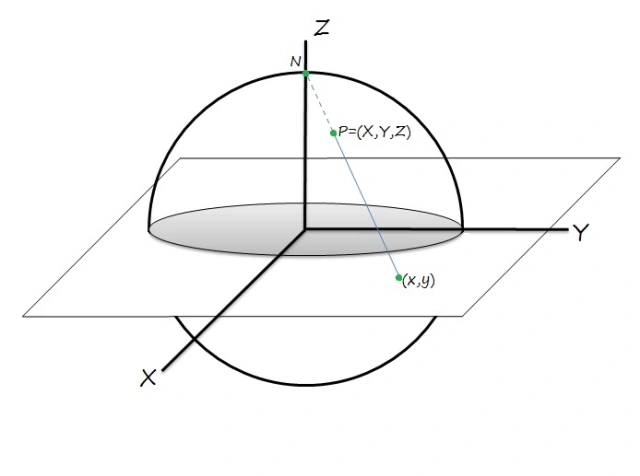
\includegraphics[width=0.5\linewidth]{P_Estereografica.png}
            \caption{Representación gráfica de la proyección estereográfica.}
        \end{figure}

        Tomamos $x=(x_1,\dots,x_n,x_{n+1})\in \bb{S}^n\setminus \{N\}$. La recta que pasa por $x$ y $N$, es:
        \begin{equation*}\begin{split}
            &(0,\dots,0,1)+\lambda\cdot \vec{(0,\dots,0,1)(x_1,\dots,x_n,x_{n+1})}
            =\\&\hspace{1cm}= (0,\dots,0,1)+\lambda\cdot (x_1,\dots,x_n,x_{n+1}-1)
            =\\&\hspace{1cm}= (\lambda x_1,\dots,\lambda x_n,1+\lambda (x_{n+1}-1))
        \end{split}\end{equation*}

        Buscamos obtener la intersección con el plano de ecuación $x_{n+1}=0$, por lo que $1+\lambda(x_{n+1}-1)=0$. Por tanto, $\lambda=\dfrac{1}{1-x_{n+1}}$. Definimos entonces la siguiente aplicación, llamada proyección estereográfica, que lleva cada punto a la correspondiente intersección descrita:
        \Func{p_e}{\bb{S}^n\setminus \{N\}}{\bb{R}^n}{(x_1,\dots,x_n,x_{n+1})}{\left(\dfrac{x_1}{1-x_{n+1}}\right),\dots,\left(\dfrac{x_n}{1-x_{n+1}}\right)}

        Calculamos ahora su inversa. Dado $(y_1,\dots,y_n)\in \bb{R}^n$, consideramos $y=(y_1,\dots,y_n, 0)\in \bb{R}^{n+1}$. La recta que pasa por $y$ y $N$, es:
        \begin{equation*}
            (0,\dots,0,1)+\mu\cdot (y_1,\dots,y_n,-1)
            = (\mu x_1,\dots,\mu x_n,1-\mu)
        \end{equation*}

        Calculamos la intersección de la recta con $\bb{S}^n$:
        \begin{gather*}
            (\mu y_1)^2 + \dots + (\mu y_n)^2 +(1-\mu)^2 = 1\\
            \mu^2(y_1^2+\dots + y_n^2) + \cancel{1} +\mu^2 -2\mu=\cancel{1}\\
            [\mu(y_1^2+\dots + y_n^2) +\mu-2]\mu=2
        \end{gather*}

        Las dos soluciones, por tanto, son $\mu=0$ (que nos da $N$, que no nos interesa), y el siguiente punto:
        \begin{equation*}
            \mu(y_1^2+\dots + y_n^2) +\mu-2 = 0 \Longrightarrow \mu=\frac{2}{1+y_1^2+\dots+y_n^2}
        \end{equation*}

        Por tanto, definimos:
        \Func{p_e^{-1}}{\bb{R}^n}{\bb{S}^n\setminus \{N\}}{(y_1,\dots,y_n)}{\left(\dfrac{2y_1}{1+y_1^2+\dots+y_n^2}\right),\dots,\left(\dfrac{2y_n}{1+y_1^2+\dots+y_n^2}, 1-\dfrac{2}{1+y_1^2+\dots+y_n^2}\right)}

        Tenemos que $p_e$ es continua, y se demuestra que $p_e^{-1}$ es su inversa, también continua. Por tanto, tenemos que ambos conjuntos son homeomorfos.

        \item Denotamos por $S=(0,\dots,0,-1)$ al polo sur de $\bb{S}^n\subset \bb{R}^{n+1}$.
        Veamos que $\bb{S}^n\setminus \{N,S\}$ es homeomorfo al cilindro $\bb{S}^{n-1}\times \bb{R}$.

        Tomamos $x=(x_1,\dots,x_n,x_{n+1})\in \bb{S}^n\setminus \{N,S\}$. La semirrecta que empieza en el origen y pasa por $x$ es:
        \begin{equation*}
            \lambda (x_1,\dots,x_n,x_{n+1}) \qquad \lambda\geq 0
        \end{equation*}

        Buscamos su intersección con el cilindro:
        \begin{equation*}
            (\lambda x_1)^2 +\dots +(\lambda x_n)^2= 1\Longrightarrow \lambda = \frac{1}{\sqrt{x_1^2+\dots+x_n^2}}
        \end{equation*}
        donde tomo el valor de la raíz positiva, ya que $\lambda\geq 0$. Además, el denominador no se anula, ya que si las primeras $n$ componentes de $x$ fuesen nulas, tendríamos que $x=N,S$, pero estos no pertenecen a nuestro conjunto.

        Por tanto, definimos la siguiente aplicación, que lleva cada punto de la esfera a la correspondiente intersección con el cilindro:
        \Func{f}{\bb{S}^n\setminus \{N,S\}}{\bb{S}^{n-1}\times \bb{R}}{(x_1,\dots,x_n,x_{n+1})}{\frac{1}{\sqrt{x_1^2+\dots +x_n^2}}\cdot (x_1,\dots,x_n,x_{n+1})}

        La inversa se construye análogamente. Consideramos $y=(y_1,\dots,y_n, y_{n+1})\in \bb{S}^n\times \bb{R}$. La semirrecta que pasa por $y$ y que empieza en el origen es:
        \begin{equation*}
            \mu (y_1,\dots,y_n,y_{n+1}) \qquad \mu\geq 0
        \end{equation*}

        Calculamos la intersección de la recta con $\bb{S}^n$:
        \begin{gather*}
            (\mu y_1)^2 + \dots + (\mu y_n)^2 +(\mu y_{n+1})^2 = 1\\
            \mu^2(y_1^2+\dots + y_n^2 + y_{n+1}^2)=1\\
            \mu^2(1 + y_{n+1}^2)=1
        \end{gather*}
        Por tanto, el valor de $\mu$ para la intersección es:
        \begin{equation*}
            \mu=\frac{1}{\sqrt{1+y_{n+1}^2}}
        \end{equation*}

        Por tanto, definimos:
        \Func{f^{-1}}{\bb{S}^{n-1}\times \bb{R}}{\bb{S}^n\setminus \{N,S\}}{(y_1,\dots,y_n,y_{n+1})}{\frac{1}{\sqrt{1+y_{n+1}^2}}\cdot (y_1,\dots, y_n,y_{n+1})}

        Tenemos que $f$ es continua, y se demuestra que $f^{-1}$ es su inversa, también continua. Por tanto, tenemos que ambos conjuntos son homeomorfos.

        \item Veamos ahora que $B(0,1)\cong \bb{R}^n$.

        TERMINAR
    \end{enumerate}
\end{ejemplo}

Debido a las caracterizaciones de la continuidad, y a la definición de homemorfismo, se tiene de forma directa la siguiente proposición.
\begin{prop}
    Sea $f:(X,\T)\to (Y,\T')$ un homeomorfismo entre dos espacios topológicos. Entonces, se tiene que:
    \begin{enumerate}
        \item $U\in \T\Longrightarrow f(U)\in \T'$,
        \item $C\in C_\T\Longrightarrow f(C)\in C_{\T'}$,
        \item $\cc{B}$ es base de la topología en $\T$ si y solo si $\cc{B}'=\{f(B)\mid B\in \cc{B}\}$ es base de la topología en $\T'$.
        \item Dado $x\in X$, se tiene que $N\in N_x \Longleftrightarrow f(N)\in N_{f(x)}$.
        \item $\beta_x$ es base de entornos de $x$ en $(X,\T)$ si y solo si $\beta_x'=\{f(V)\mid V\in \beta_x\}$ es base de entornos de $f(x)$ en $(Y,\T')$.
    \end{enumerate}
\end{prop}

\begin{definicion}
    Una propiedad se dice topológica si no cambia por homeomorfismos.
    
    Es decir, esa propiedad la cumple un espacio topológico si y solo si la cumplen todos los espacios topológicos homeomorfos a él.
\end{definicion}

Por ejemplo, y debido a lo visto anteriormente, se tiene que ser T1, T2, 1AN o 2AN son propiedades topológicas. TERMINAR.


\begin{definicion}[Embebimiento]
    Sea $f:(X,\T)\to (Y,\T')$ una aplicación entre espacios topológicos. Se dice que $f$ es un embebimiento si $f:(X,\T)\to \left(f(X),\T'_{f(X)}\right)$ es un homeomorfismo.
\end{definicion}




\section{Topología Producto}
Dados dos espacios topológicos, queremos construir una topología natural sobre $X\times Y$.


\begin{lema}
    Dados dos espacios topológicos $(X,\T), (Y,\T')$, se tiene que
    \begin{equation*}
        \cc{B} = \left\{U\times U'\subset X\times Y\mid U\in \T,~U'\in \T'\right\}
    \end{equation*}
    es base de una topología en $X\times Y$.
\end{lema}
\begin{proof}
    Usamos el Teorema \ref{teo:TopoGenerada_Bases}. Para ello, comprobamos ambas condiciones:
    \begin{enumerate}
        \item[B1)] Tenemos que ver que $X\times Y=\bigcup\limits_{B\in \cc{B}}B$.

        Como $X\in \T, Y\in \T'$, tenemos que $X\times Y\in \cc{B}$, por lo que se tiene de forma directa.

        \item[B2)] Sean $B_1,B_2\in \cc{B}$, y consideramos $(x,y)\in B_1\cap B_2$. Veamos que existe $B_3\in \cc{B}$ tal que $(x,y)\in B_3\subset B_1\cap B_2$.

        Tenemos que $B_1=U_1\times U_1', B_2=U_2\times U_2'$, con $U_1,U_2\in \T$, $U_1', U_2'\in \T'$. Como $(x,y)\in B_1\cap B_2$, tenemos que $x\in (U_1\cap U_2)$ e $y\in (U_1'\cap U_2')$. Por tanto, se tiene que $(x,y)\in (U_1\cap U_2)\times (U_1'\cap U_2')$.
        
        Definimos entonces $B_3=(U_1\cap U_2)\times (U_1'\cap U_2')$, ya que la intersección de dos abiertos es un abierto, y se tiene lo pedido.
    \end{enumerate}
\end{proof}

\begin{definicion}[Topología Producto]
    Llamamos topología producto de $(X,\T), (Y,\T')$ a la topología en $X\times Y$ que tiene por base la siguiente:
    \begin{equation*}
        \cc{B} = \left\{U\times U'\subset X\times Y\mid U\in \T,~U'\in \T'\right\}
    \end{equation*}

    A esta topología se le suele denotar por $\T\times \T'$.
\end{definicion}

Notemos que, aunque si $U\in \T, U'\in \T'$ se tenga que $U\times U'$ sí está en $\T\times \T'$, el recíproco no es cierto. Es decir, en general, un abierto de $\T\times \T'$ no es un producto de abiertos.

\begin{prop}
    Sean $(X,\T), (Y,\T')$ dos espacios topológicos. Entonces, se tiene:
    \begin{enumerate}
        \item Si $\cc{B}_X$ es una base de $\T$ y $\cc{B}_Y$ es una base de $\T'$, entonces una base de $\T\times \T'$ es:
        \begin{equation*}
            \cc{B}_{X\times Y}=\left\{B\times B'\subset X\times Y\mid B\in \cc{B}_X,~B'\in \cc{B}_Y\right\}
        \end{equation*}

        \item Si $\beta_x$ es una base de entornos de $x$ en $(X,\T)$ y $\beta_y$ es una base de entornos de $y$ en $(Y,\T')$, entonces una base de entornos de $(x,y)$ en $\T\times \T'$ es:
        \begin{equation*}
            \beta_{(x,y)}=\left\{V\times V'\subset X\times Y\mid V\in \beta_x,~V'\in \beta_y\right\}
        \end{equation*}
    \end{enumerate}
\end{prop}
\begin{proof}
    Demostramos cada uno de los resultados por separado:
    \begin{enumerate}
        \item Veamos primero que $\cc{B}_{X\times Y}\subset \T\times \T'$. Esto es evidente, ya que si $B\times B'\in \cc{B}_{X\times Y}$, entonces $B\in \T$ por ser elemento de una base de $(X,\T)$, y análogamente se tiene que $B'\in \T'$. Por tanto, $B\times B'\in \T\times \T'$.

        Ahora, probamos que si $U\in \T\times \T'$ y $(x_0,y_0)\in U$, entonces se tiene que $\exists B\times B'\in \cc{B}_{X,Y}$ tal que $(x_0,y_0)\in B\times B'\subset U$.

        Como $U\in \T\times \T'$ y $(x_0,y_0)\in U$, entonces existen por la definición de la topología producto se tienen que $\exists O\in \T,O'\in \T'$ tal que $(x_0,y_0)\in O\times O'\subset U$. Como $x_0\in O$ y $\cc{B}_X$ es una base de $(X,\T)$, entonces $\exists B\in B_X$ tal que $x_0\in B\subset O$. Análogamente, como $y_0\in O'$ y $\cc{B}_Y$ es una base de $(Y,\T')$, entonces $\exists B'\in B_Y$ tal que $y_0\in B'\subset O'$.
        
        Por tanto, tenemos que $(x_0,y_0)\in B\times B'\subset O\times O'\subset U$, tiendo entonces probado que $\cc{B}_{X\times Y}$ es una base de la topología producto.

        \item TERMINAR
    \end{enumerate}
\end{proof}


\begin{observacion}
    Como consecuencia elemental, se tiene que si $(X,\T),(Y,\T')$ son 1AN, entonces $(X\times Y, \T\times \T')$ es 1AN.

    Igualmente, si $(X,\T),(Y,\T')$ son 2AN, entonces $(X\times Y, \T\times \T')$ es 2AN.
\end{observacion}

\begin{ejemplo} Veamos algunos ejemplos de topología producto:
    \begin{enumerate}
        \item $(X,\T_t^X), (Y,\T_t^Y)$. Veamos ahora la topología producto $(X\times Y, \T_t^X\times \T_t^Y)$. Una base de $\T_t^X\times \T_t^Y$ es:
        \begin{equation*}
            \cc{B}=\{\emptyset\times \emptyset, X\times \emptyset, \emptyset\times Y, X\times Y\}=\{\emptyset, X\times Y\}
        \end{equation*}

        Además, como realizando la unión de abiertos básicos no puede generar ningún otro conjunto, tenemos que $\T_t^X\times \T^Y_t=\{\emptyset, X\times Y\}$. Por tanto, se tiene que $\T_t^X\times \T_t^Y=\T_t^{X\times Y}$.

        \item $(X,\T_{disc}^X), (Y,\T_{disc}^Y)$. Veamos ahora la topología producto $(X\times Y, \T_{disc}^X\times \T_{disc}^Y)$. Una base de $\T_{disc}^X\times \T_{disc}^Y$ es:
        \begin{equation*}
            \cc{B}=\{A\times B\mid A\subset X,~B\subset Y\}
        \end{equation*}
        
        Tenemos que cualquier punto $(x_0,y_0)$  es un abierto, ya que:
        \begin{equation*}
            \{(x_0,y_0)\} = \{x_0\}\times \{y_0\}\in \T_{disc}^X\times \T_{disc}^Y
        \end{equation*}

        Por tanto, tenemos que $\T_{disc}^{X\times Y}=\T_{disc}^X\times \T_{disc}^Y$.
    \end{enumerate}
\end{ejemplo}


Demostramos ahora el siguiente lema, que nos será de utilidad para próximos teoremas.
\begin{lema}
    Sean $p_1,q_1\in \bb{R}^n$, $p_2,q_2\in \bb{R}^m$. Entonces:
    \begin{equation*}
        \|(p_1,p_2) - (q_1, q_2)\|^2 = \|p_1-q_1\|^2 + \|p_2-q_2\|^2
    \end{equation*}
\end{lema}

\begin{prop}
    El producto de $(\bb{R}^n,\T_u^n)$ con $(\bb{R}^m,\T_u^m)$ es $(\bb{R}^{m+n},\T_u^{m+n})$. Es decir,
    \begin{equation*}
        \T_u^n\times \T_u^m = \T_u^{n+m}
    \end{equation*}
\end{prop}
\begin{proof}
    Sabemos que el siguiente conjunto es un base de la topología producto $\T_u^n\times \T_u^m$: $$\cc{B}=\{B(p_1, r_1)\times B(p_2,r_2)\mid r_1,r_2\in \bb{R}^+, p_1\in\bb{R}^^n, p_2\in \bb{R}^n\}.$$

    Queremos ver que $\cc{B}$ es también base de $\T_u^{n+m}$, lo que por el Teorema \ref{teo:TopoGenerada_Bases} implicaría que $\T_u^n\times \T_u^m = \T_u^{n+m}$.


    Probamos en primer lugar que todo elemento $B$ de $\cc{B}$ es un abierto en $\T_u^{n+m}$. Para ello, probamos que dado $q=(q_1,q_2)\in B=B(p_1,r_1)\times B(p_2,r_2)$, existe $B[(q_1,q_2), r]$ tal que $B[(q_1,q_2), r]\subset B(p_1, r_1)\times B(p_2,r_2)$.

    Definimos $r_1'=r_1-\|p_1-q_1\|$, $r_2'=r_2-\|p_2-q_2\|$, y se tiene que:
    \begin{equation*}
        B(q_1,r_1')\subset B(p_1,r_1)
        \qquad 
        B(q_2,r_2')\subset B(p_2,r_2)
    \end{equation*}
    Por tanto, $B(q_1,r_1')\times B(q_2,r_2')\subset B(p_1, r_1)\times B(p_2,r_2)$.

    Sea entonces $r=\min\{r_1',r_2'\}$. Veamos que $B[(q_1,q_2), r]\subset B(q_1,r_1')\times B(q_2,r_2')$.
    \begin{description}
        \item[$\subset)$] Sea $(x_1,x_2)\in B[(q_1,q_2), r]$. Entonces, por definición de bola y por el lema anterior, se tiene:
        \begin{equation*}
            \|x_1-q_1\|^2 + \|x_2-q_2\|^2=\|(x_1,x_2)-(q_1,q_2)\|^2<r^2
        \end{equation*}

        Por tanto, se tiene que $\|x_1-q_1\|^2<r^2\leq r_1^2$, por lo que $x_1\in B(q_1,r_1')$. Análogamente, vemos que $x_2\in B(q_2, r_2')$. Por tanto, se tiene que $(x_1,x_2)\in B(q_1,r_1')\times B(q_2,r_2')$.
    \end{description}



    Por tanto, ya tenemos que todo elemento $B$ de $\cc{B}$ es un abierto en $\T_u^{n+m}$. Veamos ahora que todo elemento de $\T_u^{n+m}$ es unión de elementos de $\cc{B}$. Para esto, basta demostrar que dados $U\in \T_u^{n+m}$ y $x=(x_1,x_2)\in U\subset \bb{R}^n\times \bb{R}^m$, existe $B\in \cc{B}$ que cumpla que $x\in B\subset U$.

    Sabemos que $\exists r>0$ tal que $B[(x_1,x_2),\bb{R}]\subset U$. Vamos a probar ahora que $B\left(x_1,\frac{r}{2}\right)\times B\left(x_2,\frac{r}{2}\right)\subset B[(x_1,x_2),r]$.
    \begin{description}
        \item[$\subset)$] Si $(y_1,y_2)\in B\left(x_1,\frac{r}{2}\right)\times B\left(x_2,\frac{r}{2}\right)$, entonces se tiene que
        \begin{equation*}
            \|y_1-x_1\|^2 < \left(\frac{r}{2}\right)^2
            \qquad
            \|y_2-x_2\|^2 < \left(\frac{r}{2}\right)^2
        \end{equation*}

        Por tanto, por el lema anterior, se tiene que:
        \begin{equation*}
            \|(y_1, y_2) - (x_1-x_2)\|^2 = \|y_1-x_1\|^2 + \|y_2-x_2\|^2 <  \left(\frac{r}{2}\right)^2 + \left(\frac{r}{2}\right)^2 < r^2
        \end{equation*}
        Por tanto, $(y_1,y_2)\in B[(x_1,x_2), r]$.
    \end{description}
\end{proof}


Tenemos además que, en la topología producto, se tiene que el producto de cerrados es cerrado (aunque al revés no se tiene). Veámoslo:
\begin{prop}
    Sean $(X,\T), (Y,\T')$ dos espacios topológicos, y consideramos $C\in C_\T$, $C'\in C_{\T'}$. Entonces, $C\times C'\in C_{\T\times \T'}$. 
\end{prop}
\begin{proof}
    Demostramos que su complementario es un abierto. 
    \begin{equation*}
        X\times Y \setminus C\times C' = (X\setminus C)\times Y \cup X\times (Y\setminus C')\in \T\times \T'
    \end{equation*}
    donde hemos visto que es un abierto de la topología producto ya que $X$ e $Y$ son abiertos en sus respectivas topologías.

    Por tanto, tenemos que $C\times C'$ es un cerrado en la topología producto.
\end{proof}